\section{Convergence Analysis}

In general, convergence proofs follow the form of analyzing a convergent
sequence $\{x_i\}_{i=1}^t$ which optimizes a function $f$. We begin by exploring the
general convergence of a convex function and prove Equation~\ref{eq:gd} when
different aspects of the curvature of $f$ are known, such as an upper bound,
lower bound, and stochastic properties under SGD.  This requires a few
definitions prior to analysis, mainly be defining convexity from a theoretical
point of view, then adding upper and lower bounds to this definition which will
aid in these proofs. 

Where convenient, we use the following notations: $x^* = \inf_x f(x)$ is the
optimal point of $f$ (which exists due to convexity), $f^* \triangleq f(x^*)$ is
the value of $f$ at the optimal point, $f_t \triangleq f(x_t)$ is the
value of $f$ at $x_t$, $\nabla f_t \triangleq \nabla f(x_t)$ is the
gradient evaluation of $f$ at $x_t$, and $\delta_t \triangleq f_t - f^*$ is the
error at $x_t$.
\begin{definition}
    A function $f: \R^n \rightarrow \R$ is \emph{convex} if for all $x, y \in
    \R^n$, for all $\lambda \in [0, 1]$,
    \begin{equation}
        \label{eq:convex}
        \lambda f(x) + (1 - \lambda)f(y) \geq f(\lambda x + (1 - \lambda)y).
    \end{equation}
\end{definition}

This definition states that any interpolation between two points
evaluated on $f$ is greater than evaluating $f$ on the interpolated points. This
provides an upper bound for a convex function over any two points and is
demonstrated by the red line in Figure~\ref{fig:convex}. Likewise, we
have that a convex function can be lower-bounded at every point by a hyperplane
which runs tangential to the function.
This concept is demonstrated by the blue line in Figure~\ref{fig:convex}. 

\begin{lemma}
    \label{lem:convex_bound}
    If a function $f$ is convex and differentiable, then for all $x, y \in \R^n$,
    \begin{equation}
        f(y) - f(x) \geq \nabla {f(x)}^\intercal (y - x)
    \end{equation}
\end{lemma}

\begin{proof}
    For $x, y \in \R^n$, Equation~\ref{eq:convex} can be restated as
    \begin{equation}
        f(y) - f(x) \geq \frac{f(x + \lambda(y - x)) - f(x)}{\lambda} \quad
        \text{for} \quad \lambda \in (0, 1].
    \end{equation}
    Taking the limit w.r.t. $\lambda$ gives us
    \begin{equation}
        \lim_{\lambda \rightarrow 0^+} \frac{f(x + \lambda(y - x)) -
        f(x)}{\lambda} = \nabla {f(x)}^\intercal(y - x)
    \end{equation}
\end{proof}

\begin{figure}[t]
    \begin{center}
        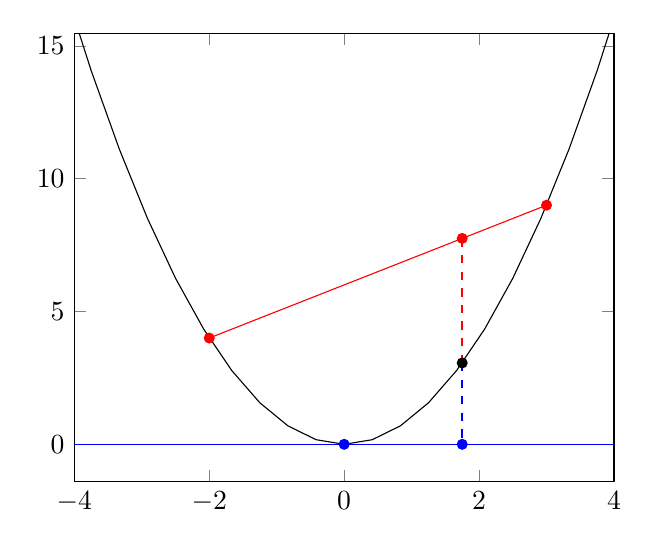
\begin{tikzpicture}[scale=1, transform shape]
            \begin{axis}[xmin=-4, xmax=4]
                \addplot[color=black] (\x, {(\x)^2});
                \addplot[color=red] coordinates { (-2,4) (3,9) };
                \fill[color=red] (axis cs:-2,4) circle (2pt and 2pt);
                \fill[color=red] (axis cs:3,9) circle (2pt and 2pt);
                \addplot[color=blue] coordinates{ (-4,0) (4,0) };
                \fill[color=blue] (axis cs:0,0) circle (2pt and 2pt);

                \addplot[color=red,dashed,thick] coordinates { (1.75,3.0625) (1.75,7.75) };
                \addplot[color=blue,dashed,thick] coordinates { (1.75,3.0625) (1.75,0) };
                \fill[color=red] (axis cs:1.75,7.75) circle (2pt and 2pt);
                \fill[color=blue] (axis cs:1.75,0) circle (2pt and 2pt);
                \fill (axis cs:1.75,3.0625) circle (2pt and 2pt);
            \end{axis}
        \end{tikzpicture}
    \end{center}
    \caption{Graph of the convex function $f(x) = x^2$. The solid red line
    indicates an interpolation between points $(-2, 4)$ and $(3, 9)$ on the
    graph while the dashed red line demonstrates the distance between the
    theoretical upper bound and the evaluation for $x = 1.75$. Likewise, the
    solid blue line indicates the hyperplane which runs tangential to the point
    $(0, 0)$ while the dashed blue line demonstrates the distance between the
    theoretical lower bound and the evaluation for the same $x$.}%
    \label{fig:convex}
\end{figure}

\subsection{Smoothness}

Smoothness is often an assumption when analyzing the convergence of gradient
descent algorithms, as it characterizes the curvature of a function quite
nicely. Most proofs benefit from the assumption that the gradient will tend to
\emph{decrease} as elements in the sequence move more towards an optimal point,
which is the property that smoothness describes.

\begin{example}
    Consider the functions $f(x) = x^2$ and $g(x) = |x|$. The function $f$ is
    much more desirable when dealing with gradient descent as $\nabla f$ scales
    with changes in $x$ as it moves closer and closer 0. The
    function $g$ yields greater difficult, since $\nabla g$ gives almost no
    information of the direction of the gradient, only yielding whether to move
    in the positive or negative direction, which will cause infinite oscillation
    if the learning rate is constant.
\end{example}


\begin{definition}
    A continuously differentiable function $f$ is $\beta$-smooth if its gradient
    is $\beta$-Lipschitz
    \begin{equation}
        \norm{\nabla f(x) - \nabla f(y)} \leq \beta \norm{x - y}.
    \end{equation}
\end{definition}

Using smoothness, one can derive both upper and lower quadratic bounds to
characterize $f$. 

\begin{lemma}[Quadratic Bounds]
    \label{lem:quadratic_bounds}
    Let $f$ be $\beta$-smooth on $\R^n$. Then for any $x, y \in \R^n$ we have 
    \begin{equation}
        \abs{f(y) - f(x) - \nabla {f(x)}^\intercal(y - x)} \leq \frac{\beta}{2}
        \norm{y - x}^2.
    \end{equation}
\end{lemma}

Lemma~\ref{lem:quadratic_bounds} can be equivalently stated as providing upper
and lower bounds on a continuously differentiable, $\beta$-smooth function $f$
at $y \in \R^n$
\begin{equation}
    - \frac{\beta}{2} \norm{y - x}^2 \leq
    f(y) - f(x) - \nabla {f(x)}^\intercal(y - x)\leq
     \frac{\beta}{2} \norm{y - x}^2
\end{equation}
where for a convex $f$, Lemma~\ref{lem:convex_bound} implies that
\begin{equation}
    \label{eq:lem4_1}
    0 \leq f(y) - f(x) - \nabla {f(x)}^\intercal (y - x) \leq
    \frac{\beta}{2} \norm{y - x}^2.
\end{equation}
In fact, when $f$ indeed is convex \emph{and} $\beta$-smooth, we can apply a
much tighter lower bound using the following lemma.

\begin{lemma}
    \label{lem:con_smo}
    Let $f$ be convex and $\beta$-smooth on $\R^n$. Then for any $x, y \in \R^n$ we have
    and
    \begin{equation}
        \label{eq:lem4_2}
\frac{1}{2\beta}
        \norm{\nabla f(y) - \nabla f(x)}^2
        \leq f(y) - f(x) - \nabla {f(x)}^\intercal (y - x) .
    \end{equation}
\end{lemma}

\begin{lemma}
    \label{lem:decreasing_parameter_update}
    Let $f$ be convex and $\beta$-smooth. Then the
    gradient descent update listed in Equation~\ref{eq:gd} with learning rates
    $\eta_t \leq \frac{1}{\beta}$ satisfies
    \begin{equation}
            \norm{x_{t + 1} - x^*}^2 \leq \norm{x_t - x^*}^2.
    \end{equation}
\end{lemma}

\begin{proof}
    By Lemma~\ref{lem:con_smo}, we can rearrange to bound the difference 
    \begin{equation}
        \label{eq:p1}
        f_t - f^* \leq -\nabla {f_t}^\intercal (x^* - x_t) - \frac{1}{2\beta}
        \norm{\nabla f_t}^2.
    \end{equation}
    Since $x^*$ was chosen s.t. $x^* = \inf_x f(x)$, we have $f(x_t) - f(x^*)
    \geq 0$ so that
    \begin{equation}
        \label{eq:p2}
        0 \leq f_t - f^* \leq -\nabla {f_t}^\intercal (x^* - x_t) - \frac{1}{2\beta}
        \norm{\nabla f_t}^2,
    \end{equation}
    and by rearranging and excluding the middle,
    \begin{equation}
        \label{eq:p3}
        \nabla {f_t}^\intercal (x^* - x_t) \leq   - \frac{1}{2\beta}
        \norm{\nabla f_t}^2.
    \end{equation}
    Note that the expansion of parameter updates based on gradient descent is
    given by
    \begin{equation}
        \label{eq:gdupdate}
        \begin{aligned}
            \norm{x_{t + 1} - x^*}^2 &= \norm{x_t - x^*}^2 - 2\eta_t {\nabla
            f_t}^\intercal (x_t - x^*) + \eta_t^2 \norm{\nabla f_t}^2. \\
        \end{aligned}
    \end{equation}
    whereby substituting Equation~\ref{eq:p3} gives us
    \begin{equation}
            \norm{x_{t + 1} - x^*}^2 \leq \norm{x_t - x^*}^2 +
            \eta_t \left(\eta_t - \frac{1}{\beta}  \right) \norm{\nabla f_t}^2
    \end{equation}
    Choice of $\eta_t \leq \frac{1}{\beta}$ implies that $\eta_t -
    \frac{1}{\beta} \leq 0$ so that 
    \begin{equation}
            \norm{x_{t + 1} - x^*}^2 \leq \norm{x_t - x^*}^2.
    \end{equation}
\end{proof}


\begin{theorem}
    \label{thm:beta_update}
    Let $f$ and $\eta_t$ be defined as in
    Lemma~\ref{lem:decreasing_parameter_update}. Then the objective difference
    satisfies
    \begin{equation}
        f_{t+1} - f^* \leq  \frac{\norm{x_1 - x^*}^2}{\sum_{i = 1}^t 1 - \frac{\beta\eta_i}{2}}
    \end{equation}
\end{theorem}


\begin{proof}
    By Lemma~\ref{lem:con_smo}, the progress in objective function satisfies
    \begin{equation}
        f_{t+1} - f_t \leq -\eta_t \left( 1 - \eta_t \frac{\beta}{2}
        \right)\norm{\nabla f_t}^2.
    \end{equation}
    We can add and subtract $f^*$ to determine a 
    forumlation relative to $f^*$
    \begin{equation}
        (f_{t+1} {- f^*}) - (f_t {- f^*}) = \delta_{t+1} - \delta_t \leq -\eta_t \left( 1 - \eta_t \frac{\beta}{2}
        \right)\norm{\nabla f_t}^2.
    \end{equation}
    By Lemma~\ref{lem:convex_bound} we have that 
    \begin{equation}
        \delta_t =  f_t - f^* \leq -\nabla f_t^\intercal (x^* - x_t),
    \end{equation}
    which by the Cauchy-Schwartz inequality gives us
    \begin{equation}
        \delta_t^2 \leq {\left(\nabla f_t^\intercal (x^* - x_t)\right)}^2 \leq
        \norm{\nabla f_t}^2\norm{x_t - x^*}^2,
    \end{equation}
    which can be plugged back into Equation~\ref{eq:dt1} to get
    \begin{equation}
        \delta_{t+1} - \delta_t \leq -\eta_t \left( 1 - \eta_t \frac{\beta}{2}
        \right) { \frac{\delta_t^2}{\norm{x_t - x^*}^2}}.
    \end{equation}
    The difference in parameter updates given by
    Lemma~\ref{lem:decreasing_parameter_update} tells us 
    \begin{equation}
        \label{eq:deltabound}
        \delta_{t+1} - \delta_t \leq -\eta_t \left( 1 - \eta_t \frac{\beta}{2}
        \right) \frac{\delta_t^2}{ \norm{x_1 - x^*}^2}.
    \end{equation}
    By dividing both sides by $\delta_{t + 1}\delta_t$, we can make use of the
    fact that since $f_{t+1} \leq f_t \implies \delta_{t+1} \leq \delta_t$, then
    the ratio satisfies the inequality
    \begin{equation}
        \frac{\delta_t}{\delta_{t+1}} \geq 1
    \end{equation}
    which gives us the left side of Equation~\ref{eq:deltabound}  as
    \begin{equation}
        \frac{\delta_{t+1} - \delta_t}{ \delta_{t+1}\delta_t} =
        \frac{1}{\delta_t} - \frac{1}{\delta_{t + 1}}
    \end{equation}
    and the right side as 
    \begin{equation}
        \begin{aligned}
        -\eta_t \left( 1 - \eta_t \frac{\beta}{2} \right) \frac{\delta_t^2}{\norm{x_1 - x^*}^2}
            {\frac{1}{\delta_{t+1}\delta_t} } &= 
        -\eta_t \left( 1 - \eta_t \frac{\beta}{2} \right)
        \frac{1}{\norm{x_1 - x^*}^2}
            {\frac{\delta_t}{\delta_{t+1}} } \\ &\leq
        -\eta_t \left( 1 - \eta_t \frac{\beta}{2} \right)
        \frac{ 1}{\norm{x_1 - x^*}^2}.
        \end{aligned}
    \end{equation}
    Putting these two together yields the equation
    \begin{equation}
        \frac{1}{\delta_t} - \frac{1}{\delta_{t + 1}} \leq
        -\eta_t \left( 1 - \eta_t \frac{\beta}{2} \right)
        \frac{1}{\norm{x_1 - x^*}^2}.
    \end{equation}
    which forms the telescopic series
    \begin{equation}
        \sum^{t}_{i=1} \frac{1}{\delta_i} - \frac{1}{\delta_{i + 1}} \leq
        -\sum^{t}_{i=1} \eta_i \left( 1 - \eta_i \frac{\beta}{2} \right)
        \frac{1}{\norm{x_1 - x^*}^2},
    \end{equation}
    or put more simply
    \begin{equation}
       \frac{1}{\delta_1} - \frac{1}{\delta_{t + 1}} \leq
        -\sum^{t}_{i=1} \eta_i \left( 1 - \eta_i \frac{\beta}{2} \right)
        \frac{1}{\norm{x_1 - x^*}^2}.
    \end{equation}
    Since $\delta_1 \geq \delta_{t+1} \geq 0$,
    \begin{equation}
        - \frac{1}{\delta_{t+1}} \leq \frac{1}{\delta_1} - \frac{1}{\delta_{t+1}}.
    \end{equation}
    By using this, taking the negative reciprocal, and plugging back in the
    definition of $\delta_t$, we get the desired equation
    \begin{equation}
      f_{t + 1} - f^* \leq
        \frac{\norm{x_1 - x^*}^2}{\sum^{t}_{i=1} \eta_i \left( 1 - \eta_i \frac{\beta}{2} \right)}.
    \end{equation}
\end{proof}

\begin{corollary}
    With constant learning rate $\eta_i = \frac{1}{\beta}$, residual error in
    parameter updates are bounded by
    \begin{equation}
        f_{t+1} - f^* \leq \frac{2\beta}{t} \norm{x_0 - x^*}^2
    \end{equation}
\end{corollary}

\begin{proof}
    Substitute the learning update into Theorem~\ref{thm:beta_update} to get 
    \begin{equation}
        \begin{aligned}
            f_{t + 1} - f^* &\leq \frac{\norm{x_1 - x^*}^2}{\sum^{t}_{i=1} \frac{1}{2\beta}} \\
            &= \frac{\norm{x_1 - x^*}^2}{\frac{t}{2\beta}} \\
            &= \frac{2\beta}{t}  \norm{x_1 - x^*}^2
        \end{aligned}
    \end{equation}
\end{proof}


\subsection{Strong Convexity}

\begin{definition}
    A function $f$ is $\alpha$-strongly convex if for $\alpha > 0$ and $x \in
    \R^n$
    \begin{equation}
        f(x) - \frac{\alpha}{2}\norm{x}^2   
    \end{equation}
    is convex.
\end{definition}

Strong convexity allows us to apply a tighter lower bound to that derived in
Lemmas~\ref{lem:convex_bound} and~\ref{lem:con_smo} using the following Lemma.

\begin{lemma}
    Let $f$ be $\alpha$-strong convex. Then for all $x, y \in \R^n$ we have 
    \begin{equation}
\frac{\alpha}{2}
        \norm{y - x}^2
        \leq f(y) - f(x) - \nabla {f(x)}^\intercal(y - x)     \end{equation}
\end{lemma}

\begin{lemma}[Coercivity of the Gradient]
    Let $f$ be $\beta$-smooth and $\alpha$-strongly convex. Then for all $x$ and
    $y$ we have
    \begin{equation}
        {(\nabla f(x) - \nabla f(y))}^\intercal (x - y) \geq
        \frac{\alpha\beta}{\alpha + \beta} \norm{x - y}^2 + \frac{1}{\alpha +
        \beta} \norm{\nabla f(x) - \nabla f(y)}^2.
    \end{equation}
\end{lemma}

\begin{theorem}[General Convergence]
    Let $f$ be $\beta$-smooth  and $\alpha$-strongly convex. Then the
    gradient descent update listed in Equation~\ref{eq:gd} with learning rates
    $\eta_i$ satisfies
    \begin{equation}
        f_{t+1} - f^* \leq \frac{\beta}{2} \norm{x_1 - x^*}^2\prod_{i = 1}^t {\left( 1 - \eta_i \beta
        \right)}^{2} .
    \end{equation}
\end{theorem}

\begin{proof}
    Since $f$ is $\beta$-smooth, convex, and
    $\nabla f^* = 0$ by definition, Lemma~\ref{lem:con_smo} yields
    \begin{equation}
        \label{eq:to_bound}
        f_t - f^* \leq \frac{\beta}{2} \norm{x_t - x^*}^2.
    \end{equation}
    Additionally, we get from definition of $\beta$-smooth that 
    \begin{equation}
        \norm{\nabla f_t} \leq \beta \norm{x_t - x^*}.
    \end{equation}
    We can then bound Equation~\ref{eq:to_bound} by bounding $\norm{x_t - x^*}^2$.
    \begin{equation}
        \begin{aligned}
            \norm{x_{t + 1} - x^*}^2 &= {\left( x_{t} - \eta_t \nabla f_t - x^*
            \right)}^\intercal \left( x_{t} - \eta_t \nabla f_t - x^* \right)
            \\
            &= {\left( (x_{t} - x^*) - \eta_t \nabla f_t 
            \right)}^\intercal \left( (x_{t}-x^*) - \eta_t \nabla f_t \right)
            \\
            &= \norm{x_t - x^*}^2 - 2\eta_t {\nabla
            f_t}^\intercal (x_t - x^*) + \eta_t^2 \norm{\nabla f_t}^2 \\
            &= \norm{x_t - x^*}^2 - 2\eta_t {[\nabla
            f_t - \nabla f(x^\star)]}^\intercal (x_t - x^*) + \eta_t^2
            \norm{\nabla f_t}^2 \\
            &\leq \left[ 1 - 2\eta_t \frac{\alpha \beta}{\alpha + \beta}
            \right]\norm{x_t - x^*}^2 + \left[  \eta_t^2  - 2\eta_t\frac{1}{\alpha +
            \beta} \right]\norm{\nabla f_t}^2\\
            &= \left[ 1 - 2\eta_t \frac{\alpha \beta}{\alpha + \beta}
              + \eta_t^2\beta^2  - 2\eta_t\frac{\beta^2}{\alpha +
            \beta} \right]\norm{x_t - x^*}^2 \\
            &= \left[ 1 - 2\eta_t \beta 
              + \eta_t^2\beta^2  \right]\norm{x_t - x^*}^2 \\
            &= {\left( 1 -  \eta_t\beta  \right)}^2\norm{x_t - x^*}^2 \\
            &\leq \frac{\beta}{2} \norm{x_1 - x^*}^2\prod_{i = 1}^t {\left( 1 - \eta_i \beta
        \right)}^{2} 
        \end{aligned}
    \end{equation}
\end{proof}

Although the previous equation derives a setting for the general convergence of
such a function, we can get much stricter bounds under specified learning rates.

\begin{theorem}[Convergence for $\eta = 2 / (\alpha + \beta)$]
    Let $f$ be $\beta$-smooth and $\alpha$-strongly convex. Then the
    gradient descent update listed in Equation~\ref{eq:gd} with constant learning rate
    $\eta = \frac{2}{\alpha + \beta} $ satisfies
    \begin{equation}
        f_{t+1} - f^* \leq \frac{\beta}{2} \exp \left( - \frac{4t}{\kappa
        + 1} \right) \norm{x_1 - x^*}^2.
    \end{equation}
\end{theorem}

\begin{proof}
    We use the same steps leading up to the previous proof, and begin
    modifications where the two differ. Let $\kappa = \frac{\beta}{\alpha} $ be
    the \emph{condition number}.
    \begin{equation}
        \begin{aligned}
            \norm{x_{t + 1} - x^*}^2 
            &\leq \left[ 1 - 2\eta \frac{\alpha \beta}{\alpha + \beta}
            \right]\norm{x_t - x^*}^2 + \left[  \eta^2  - 2\eta\frac{1}{\alpha +
            \beta} \right]\norm{\nabla f_t}^2\\
            &= \left[ 1 - 2\eta \frac{\alpha \beta}{\alpha + \beta}
            \right]\norm{x_t - x^*}^2 \\
            &= {\left( \frac{\kappa - 1}{\kappa + 1} 
            \right)}^2\norm{x_t - x^*}^2 \\
            &\leq {\left( \frac{\kappa - 1}{\kappa + 1} 
            \right)}^{2t}\norm{x_1 - x^*}^2 \\
            &\leq \exp \left( -\sum_{i = 1}^{2t} \frac{2}{\kappa
        + 1} \right) \norm{x_1 - x^*}^2 \\
            &= \exp \left( - \frac{4t}{\kappa
        + 1} \right) \norm{x_1 - x^*}^2
        \end{aligned}
    \end{equation}
\end{proof}

\subsection{Stochastic Gradient Descent}%
\label{sub:stochastic_gradient_descent}

Stochastic gradient descent slightly differs from Equation~\ref{eq:gd} in that
instead of a deterministic valued $\nabla f$, we consider the case where the
optimization task is 
\begin{equation}
    \inf_x f(x) = \E[F(x, \xi)]
\end{equation}
where $F:\R^n \times \R^d \rightarrow \R$ is continuously differentiable, $\xi
$ is a random variable supported on the distribution $\Xi \subseteq \R^d$, and we have generally that
either $F(\cdot, \xi)$ is not given explicitly and/or the distribution of $\Xi$
is unknown. This is the case for most machine learning problems and hence is
important to study alongside general gradient descent methods. In these cases,
we may only rely upon the known properties of $f$ (e.g.\ $\beta$-smooth,
convexity, etc) and the noisy information in $\nabla f$ to optimize parameters
in this form. We assume that the noisy gradients of $f$ can be
given to us by a Stochastic First-Order Oracle (SFO) in the form of $g(x, \xi)$.
From hereafter, we use the notation $g_t \triangleq g(x_t, \xi_t)$.
This random variable $g$ is assumed to have the properties that it is 
\begin{enumerate}
    \item an unbiased estimate \begin{equation}\E[g_t] = \nabla
    f_t,\end{equation}
    \item and has an upper bound on the noise distribution, i.e. for some
        $\sigma > 0$, the max noise level of the gradient estimation is
        \begin{equation}
            \E \left[ \norm{g_t - \nabla f_t}^2 \right] \leq \sigma^2.
        \end{equation}
\end{enumerate}


\begin{proof}
    Let $\Delta_t = g_t - \nabla f_t$. Lemma~\ref{lem:quadratic_bounds} gives us
    the inequality
    \begin{equation}
        \begin{aligned}
            f_{t+1} - f_t &\leq - \eta_t {\nabla f_t}^\intercal g_t +
            \eta_t^2\frac{\beta}{2} \norm{g_t}^2 \\
            &= - \eta_t \norm{\nabla f_t}^2 - \eta_t \nabla f_t^\intercal \Delta_t +
            \eta_t^2\frac{\beta}{2} \norm{g_t}^2
        \end{aligned}
    \end{equation}
    By taking the expectation of both sides and noting that $\E[\Delta_t |
    x_t] = \nabla f_t - \nabla f_t = 0$, we get
    \begin{equation}
        \begin{aligned}
            \E[f_{t+1} | x_t] - f_t &\leq - \eta_t \norm{\nabla f_t}^2 +
            \eta_t^2\frac{\beta}{2} \E[\norm{g_t}^2 | x_t]
        \end{aligned}
    \end{equation}
    where the last term expands out to
    \begin{equation}
        \begin{aligned}
            \E[\norm{g_t}^2 | x_t] &= \E[\norm{\Delta_t + \nabla f_t}^2 | x_t]
            \\
            &= \E[\norm{\Delta_t + \nabla f_t}^2 | x_t] \\
            &= \E[\norm{\Delta_t}^2 | x_t] + 2 \E[\nabla f_t^\intercal \Delta_t
            | x_t] + \E[\norm{\nabla f_t}^2 | x_t] \\
            &= \norm{\nabla f_t}^2 + \sigma^2
        \end{aligned}
    \end{equation}
    yielding the final equation
    \begin{equation}
        \begin{aligned}
            \E[f_{t+1} | x_t] - f_t &\leq - \eta_t \left( 1 - \eta_t
            \frac{\beta}{2}  \right) \norm{\nabla f_t}^2 +
             \eta_t^2\sigma^2 \frac{\beta}{2} 
        \end{aligned}
    \end{equation}
\end{proof}
